\documentclass[../../main.tex]{subfiles}
\graphicspath{{../../image/}{../../figure/}}
\begin{document}

\section{波扇的相互作用}\label{section:ch09-波扇的相互作用}

到目前为止,我们利用守恒律方程组在时空坐标均匀拉伸下的不变性,实施揭示解局部结构的拉伸。然而,人们也可在尺度的另一端操作,对时空坐标作收缩,从而从远离原点处观察解。初值 $U_{0}(x)$ 当 $x\to-\infty$、$x\to\infty$ 时充分快地收敛到状态 $U_{L}$、$U_{R}$,合理地产生出从远处看像居大波扇那样把左状态 $U_{L}$ 与右状态 $U_{R}$ 连接起来的解。事实上,正如后文各章所示,这确为真。的确,一维双曲守恒律方程组的本质特征似乎在于:Riemann 问题描述了时间尺度两端解的渐近性态——瞬时的与长期的。

此处目的是讨论一个相关问题,正如我们将在第 XIII 章所见,它在随机选择法构造解中起核心作用。我们考虑三个波扇:第一个把左状态 $U_{L}$ 与右状态 $U_{M}$ 相连;第二个把左状态 $U_{M}$ 与右状态 $U_{R}$ 相连;第三个把左状态 $U_{L}$ 与右状态 $U_{R}$ 相连。它们可由各自左状态 $U_{L}$、$U_{M}$、$U_{L}$ 连同相应波振幅 $n$-数组 $\alpha=(\alpha_{1},\dots,\alpha_{n})$、$\beta=(\beta_{1},\dots,\beta_{n})$、$\varepsilon=(\varepsilon_{1},\dots,\varepsilon_{n})$ 标识。基于上述论证,自然把波扇 $\varepsilon$ 视为左波扇 $\alpha$ 与右波扇 $\beta$ 相互作用的结果。回忆\eqref{align:ch09-9-3-4}, $U_{M}=\Omega(\alpha;U_{L})$, $U_{R}=\Omega(\beta;U_{M})$, $U_{R}=\Omega(\varepsilon;U_{L})$,由此推出
\begin{align}
\Omega(\varepsilon;U_{L})=\Omega(\beta;\Omega(\alpha;U_{L})).
\label{align:ch09-9-9-1}
\end{align}
这隐式确定关系
\begin{align}
\varepsilon=E(\alpha;\beta;U_{L}).
\label{align:ch09-9-9-2}
\end{align}
我们的任务是研究函数 $E$ 在 $(0;0;U_{L})$ 附近的性质。

先考虑特征族要么真正非线性\eqref{align:ch07-特征向量规范化}要么线性退化\eqref{align:ch07-线性退化条件}的方程组,此时波曲线 $\Phi_{i}$ 从而 $\Omega$ 与 $E$ 都是 $C^{2,1}$ 函数。由 $\Omega(0;\bar{U})=\bar{U}$,
\begin{align}
E(\alpha;0;U_{L})=\alpha,\qquad E(0;\beta;U_{L})=\beta,
\label{align:ch09-9-9-3}
\end{align}
由此
\begin{align}
\frac{\partial E_{k}}{\partial\alpha_{i}}(0;0;U_{L})=\delta_{ik},\qquad\frac{\partial E_{k}}{\partial\beta_{j}}(0;0;U_{L})=\delta_{jk},
\label{align:ch09-9-9-4}
\end{align}
即 Kronecker $\delta$。

从恒等式
\begin{align}
&E(\alpha;\beta;U_{L})-E(\alpha;0;U_{L})-E(0;\beta;U_{L})+E(0;0;U_{L})\nonumber\\
&=\sum_{i,j=1}^{n}\big\{E(\alpha_{1},\dots,\alpha_{i},0,\dots,0;0,\dots,0,\beta_{j},\dots,\beta_{n};U_{L})\nonumber\\
&\qquad-E(\alpha_{1},\dots,\alpha_{i-1},0,\dots,0;0,\dots,0,\beta_{j},\dots,\beta_{n};U_{L})\nonumber\\
&\qquad-E(\alpha_{1},\dots,\alpha_{i},0,\dots,0;0,\dots,0,\beta_{j+1},\dots,\beta_{n};U_{L})\nonumber\\
&\qquad+E(\alpha_{1},\dots,\alpha_{i-1},0,\dots,0;0,\dots,0,\beta_{j+1},\dots,\beta_{n};U_{L})\big\},
\label{align:ch09-9-9-5}
\end{align}
立得
\begin{align}
E(\alpha;\beta;U_{L})=\alpha+\beta+\sum_{i,j=1}^{n}\alpha_{i}\beta_{j}\int_{0}^{1}\int_{0}^{1}\frac{\partial^{2}E}{\partial\alpha_{i}\partial\beta_{j}}\,\mathrm{d}\rho\,\mathrm{d}\sigma,
\label{align:ch09-9-9-6}
\end{align}
其中 $\partial^{2}E/\partial\alpha_{i}\partial\beta_{j}$ 在 $(\alpha_{1},\dots,\alpha_{i-1},\rho\alpha_{i},0,\dots,0;0,\dots,0,\sigma\beta_{j},\beta_{j+i},\dots,\beta_{n};U_{L})$ 处取值。

称波扇 $\alpha$ 的 $i$-波与波扇 $\beta$ 的 $j$-波\emph{相互接近},当满足(a) $i>j$,或(b) $i=j$、$i$-特征族真正非线性且 $\alpha_{i}$、$\beta_{i}$ 中至少一个为负(即对应激波)。波扇 $\alpha$ 与 $\beta$ 的\emph{波相互作用量}由下式度量:
\begin{align}
D(\alpha,\beta)=\sum_{\mathrm{app}}|\alpha_{i}||\beta_{j}|,
\label{align:ch09-9-9-7}
\end{align}
其中 $\sum_{\mathrm{app}}$ 表示对所有相互接近波对求和。关键观察是:当波扇 $\alpha$ 与 $\beta$ 不含任何相互接近波,即 $D(\alpha,\beta)=0$ 时,波扇 $\varepsilon$ 由左波扇 $\alpha$ 与右波扇 $\beta$ "粘合"而成,即 $\varepsilon=\alpha+\beta$。特别地,当 $\alpha$ 的 $i$-波与 $\beta$ 的 $j$-波不相互接近时,要么因 $i<j$,要么因 $i=j$ 且 $\alpha_{i}$、$\beta_{i}$ 都为正(即都对应稀疏波),则
\begin{align}
E(\alpha_{1},\dots,\alpha_{i},0,\dots,0;0,\dots,0,\beta_{j},\dots,\beta_{n};U_{L})
=(\alpha_{1},\dots,\alpha_{i},0,\dots,0)+(0,\dots,0,\beta_{j},\dots,\beta_{n}),
\label{align:ch09-9-9-8}
\end{align}
由此\eqref{align:ch09-9-9-6}右端求和中相应 $(i,j)$ 项为零。于是\eqref{align:ch09-9-9-6}化为
\begin{align}
\varepsilon=\alpha+\beta+\sum_{\mathrm{app}}\alpha_{i}\beta_{j}\frac{\partial^{2}E}{\partial\alpha_{i}\partial\beta_{j}}(0;0;U_{L})+D(\alpha,\beta)O(|\alpha|+|\beta|).
\label{align:ch09-9-9-9}
\end{align}

\eqref{align:ch09-9-9-9}的显著特征(将在第 XIII 章起关键作用)是:波相互作用效应仅由相互接近波对诱发,在无此类波对时消失。为确定领头的二阶相互作用项,先对\eqref{align:ch09-9-9-1}关于 $\beta_{j}$ 求导并令 $\beta=0$。利用\eqref{align:ch09-9-3-8},得
\begin{align}
\sum_{k=1}^{n}\frac{\partial E_{k}}{\partial\beta_{j}}(\alpha;0;U_{L})\frac{\partial\Omega}{\partial\varepsilon_{k}}(E(\alpha;0;U_{L});U_{L})=R_{j}(\Omega(\alpha;U_{L})).
\label{align:ch09-9-9-10}
\end{align}
再对\eqref{align:ch09-9-9-10}关于 $\alpha_{i}$ 求导并令 $\alpha=0$。回忆我们只关心 $\alpha$ 的 $i$-波与 $\beta$ 的 $j$-波相互接近的情形,特别有 $i\geqslant j$。因而利用\eqref{align:ch09-9-9-3}、\eqref{align:ch09-9-9-4}、\eqref{align:ch09-9-3-8}、\eqref{align:ch09-9-3-9}、\eqref{align:ch09-9-3-10}与\eqref{align:ch07-Lie括号定义},得
\begin{align}
\sum_{k=1}^{n}\frac{\partial^{2}E_{k}}{\partial\alpha_{i}\partial\beta_{j}}(0;0;U_{L})R_{k}(U_{L})=-[R_{i}(U_{L}),R_{j}(U_{L})],
\label{align:ch09-9-9-11}
\end{align}
由此
\begin{align}
\frac{\partial^{2}E_{k}}{\partial\alpha_{i}\partial\beta_{j}}(0;0;U_{L})=-L_{k}(U_{L})[R_{i}(U_{L}),R_{j}(U_{L})].
\label{align:ch09-9-9-12}
\end{align}
特别地,当方程组配有 Riemann 不变量坐标系统时,在归一化\eqref{align:ch07-Riemann规范化}下 Lie 括号 $[R_{i},R_{j}]$ 为零(见\eqref{align:ch07-Lie括号零}),从而\eqref{align:ch09-9-9-9}中二次项消失。

合并\eqref{align:ch09-9-9-9}与\eqref{align:ch09-9-9-12},得

\begin{theorem}\label{theorem:ch09-波扇相互作用}
在特征族要么真正非线性要么线性退化的方程组中,设 $\varepsilon=(\varepsilon_{1},\dots,\varepsilon_{n})$ 是左波扇 $\alpha=(\alpha_{1},\dots,\alpha_{n})$ 与右波扇 $\beta=(\beta_{1},\dots,\beta_{n})$ 相互作用生成的波扇。则
\begin{align}
\varepsilon=\alpha+\beta-\sum_{i>j}\alpha_{i}\beta_{j}L[R_{i},R_{j}]+D(\alpha,\beta)O(|\alpha|+|\beta|),
\label{align:ch09-9-9-13}
\end{align}
其中 $L$ 表示以左特征向量 $L_{k}$ 为第 $k$ 行向量的 $n\times n$ 矩阵, $D(\alpha,\beta)$ 是 $\alpha$ 与 $\beta$ 的波相互作用量。当方程组配有 Riemann 不变量坐标系统时,二次项消失。
\end{theorem}

现考虑特征族可能仅分段真正非线性的方程组的波相互作用,此时入射与出射波扇将含复合 $i$-波,每个复合 $i$-波由有限序列的初等 $i$-波(即 $i$-激波与 $i$-稀疏波)组成。有两个障碍需克服。第一个是技术性的:如\cref{section:ch09-一般严格双曲方程组}所注,波曲线 $\Phi_{i}$ 从而函数 $\Omega$ 与 $E$ 现在可能仅 Lipschitz 连续。因而上述\eqref{align:ch09-9-9-13}的推导不再有效,因为它依赖 Taylor 展开。然而最严重的困难是如何识别相互接近波。显然,左 $i$-波与右 $j$-波当 $i>j$ 时相互接近,当 $i<j$ 时不接近。当两入射波属于同一特征族时情形更微妙。回忆在真正非线性情形,两入射 $i$-波当至少一个为激波时总是相互接近,当两者皆为稀疏波时从不接近。相比之下,此处两入射 $i$-波扇既可含不接近的 $i$-激波对,也可含接近的 $i$-稀疏波对。因而此类方程组的\cref{theorem:ch09-波扇相互作用}类比相当复杂:

\begin{theorem}\label{theorem:ch09-分段非线性波扇相互作用}
在特征族要么分段真正非线性要么线性退化的方程组中,设 $\varepsilon=(\varepsilon_{1},\dots,\varepsilon_{n})$ 是左波扇 $\alpha=(\alpha_{1},\dots,\alpha_{n})$ 与右波扇 $\beta=(\beta_{1},\dots,\beta_{n})$ 相互作用生成的波扇。则
\begin{align}
\varepsilon=\alpha+\beta+O(1)D(\alpha,\beta),
\label{align:ch09-9-9-14}
\end{align}
其中
\begin{align}
D(\alpha,\beta)=\sum\theta|\gamma||\delta|,
\label{align:ch09-9-9-15}
\end{align}
求和遍历所有初等波对,其中振幅为 $\gamma$ 的第一个波是从左入射的 $i$-波扇的一部分,振幅为 $\delta$ 的第二个波是从右入射的 $j$-波扇的一部分;权重因子 $\theta$ 按下列规则选取。
\begin{enumerate}
\item 当 $i<j$ 时, $\theta=0$。
\item 当 $i>j$,或 $i=j$ 且 $\gamma\delta<0$ 时, $\theta=1$。
\item 当 $i=j$ 且 $\gamma\delta>0$ 时, $\theta$ 确定如下:
\begin{enumerate}
\item 若两入射初等波皆为 $i$-激波,速度分别为 $\sigma_{L}$、$\sigma_{R}$,则
\begin{align}
\theta=(\sigma_{L}-\sigma_{R})^{+}.
\label{align:ch09-9-9-16a}
\end{align}
\item 若从左入射的初等波是速度为 $\sigma_{L}$ 的 $i$-激波,而从右入射的初等波是连接状态 $U_{R}$ 与 $V_{i}(\tau_{R};U_{R})$ 的 $i$-稀疏波,则
\begin{align}
\theta=\frac{1}{\tau_{R}}\int_{0}^{\tau_{R}}[\sigma_{L}-\lambda_{i}(V_{i}(\tau;U_{R}))]^{+}\,\mathrm{d}\tau.
\label{align:ch09-9-9-16b}
\end{align}
\item 若从左入射的初等波是连接状态 $U_{L}$ 与 $V_{i}(\tau_{L};U_{L})$ 的 $i$-稀疏波,而从右入射的初等波是速度为 $\sigma_{R}$ 的 $i$-激波,则
\begin{align}
\theta=\frac{1}{\tau_{L}}\int_{0}^{\tau_{L}}[\lambda_{i}(V_{i}(\tau';U_{L}))-\sigma_{R}]^{+}\,\mathrm{d}\tau'.
\label{align:ch09-9-9-16c}
\end{align}
\item 若两入射初等波皆为 $i$-稀疏波,右侧连接 $U_{R}$ 与 $V_{i}(\tau_{R};U_{R})$,左侧连接 $U_{L}$ 与 $V_{i}(\tau_{L};U_{L})$,则
\begin{align}
\theta=\frac{1}{\tau_{L}\tau_{R}}\int_{0}^{\tau_{L}}\int_{0}^{\tau_{R}}[\lambda_{i}(V_{i}(\tau';U_{L}))-\lambda_{i}(V_{i}(\tau;U_{R}))]^{+}\,\mathrm{d}\tau\,\mathrm{d}\tau'.
\label{align:ch09-9-9-16d}
\end{align}
\end{enumerate}
\end{enumerate}
\end{theorem}

\textbf{证明梗概。}此处目的是解释权重因子 $\theta$ 为何以及如何起作用。对于从左入射的 $i$-初等波与从右入射的 $j$-初等波相互作用的情形,基于本节前面的讨论,容易理解为何 $i<j$ 时 $\theta=0$、$i>j$ 时 $\theta=1$;真正的困难出现在 $i=j$ 时。

应注意,若接受\eqref{align:ch09-9-9-16a}为相互作用激波情形权重因子 $\theta$ 的正确值,则涉及稀疏波的\eqref{align:ch09-9-9-16b}、\eqref{align:ch09-9-9-16c}、\eqref{align:ch09-9-9-16d}可如下导出。任一 $i$-稀疏波可视作无穷多个(不容许的) $i$-稀疏激波组成的波扇,每个振幅与特征速度都无穷小,然后通过用\eqref{align:ch09-9-9-16a}清点这些无穷小激波的贡献,来计算它对波相互作用量的贡献。

下面将证明,当每个入射波扇由单个 $i$-激波组成时,\eqref{align:ch09-9-9-16a}确为权重因子的正确值。一般入射波扇的证明较长且技术性强,可在\cref{section:ch09-注记}所引文献中找到。

设从左入射的 $i$-激波连接 $U_{L}$ 与 $U_{M}$,振幅 $\gamma$,速度 $\sigma_{L}$;从右入射的 $i$-激波连接 $U_{M}$ 与 $U_{R}$,振幅 $\delta$,速度 $\sigma_{R}$。由 Lax $E$ 条件, $\sigma_{L}\geqslant\lambda_{i}(U_{M})\geqslant\sigma_{R}$,故两入射激波的相对速度 $\theta=\sigma_{L}-\sigma_{R}$ 非负。注意 $\theta$ 本质上度量这两激波间的夹角;相应地, $\theta$ 称为\emph{入射角}。

两入射激波的碰撞将产生出射波扇 $\varepsilon=(\varepsilon_{1},\dots,\varepsilon_{n})$,它由求解端状态为 $U_{L}$、$U_{R}$ 的 Riemann 问题确定。为简单起见,设 $\varepsilon$ 的 $i$-波扇由单个 $i$-激波组成,连接 $\bar{U}_{L}$ 与 $\bar{U}_{R}$,振幅 $\varepsilon_{i}$,速度 $\sigma$。

有两种不同的可能波构型,如图\ref{figure:ch09-激波碰撞}中(a)、(b)所示,取决于 $\gamma$ 与 $\delta$ 同号还是异号。两种情形下都有 $\varepsilon=\varepsilon(\gamma,\delta;U_{L})$,其中 $\varepsilon(0,\delta;U_{L})=(0,\dots,0,\delta,0,\dots,0)$, $\varepsilon(\gamma,0;U_{L})=(0,\dots,0,\gamma,0,\dots,0)$。因而 $\varepsilon_{i}=\gamma+\delta+O(\gamma\delta)$,而对 $j\neq i$ 有 $\varepsilon_{j}=O(\gamma\delta)$。

\begin{figure}[ht]
\centering
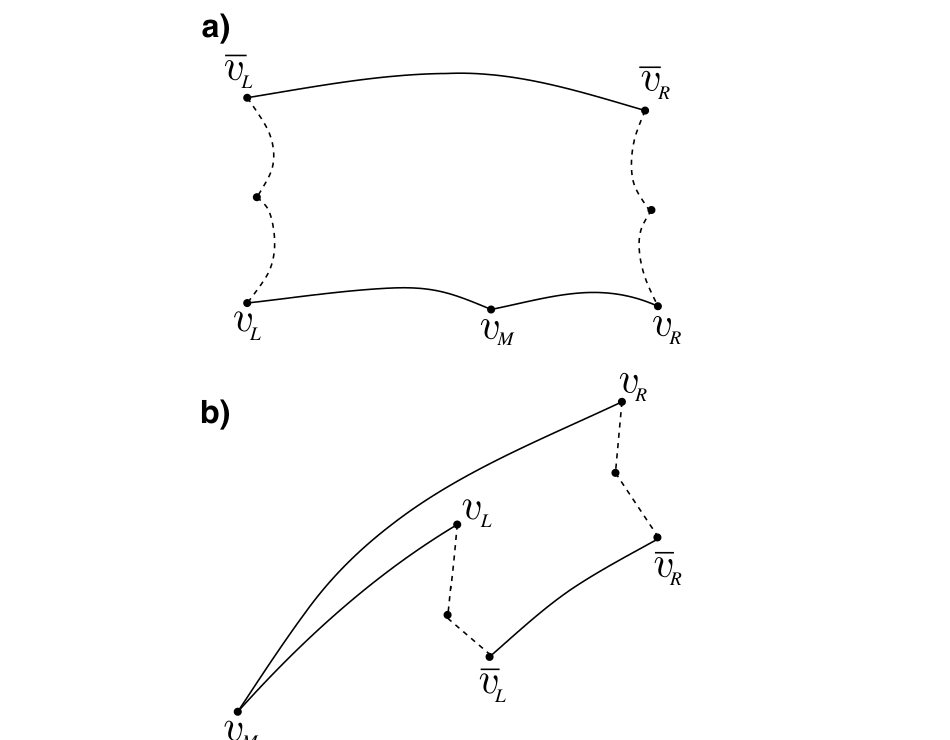
\includegraphics[width=0.62\textwidth]{ch09-fig09-01.png}
\caption{两入射 $i$-激波碰撞的两种波构型:(a) $\gamma\delta>0$;(b) $\gamma\delta<0$。}
\label{figure:ch09-激波碰撞}
\end{figure}

对波相互作用量而言, $O(\gamma\delta)$ 这一相对粗糙的界已足以满足第 XIII 章中的预期应用,当 $\gamma\delta<0$ 时,因为此时线性项中的抵消占主导。相比之下,当 $\gamma\delta>0$ 时需要更精细的估计。正是在此处,入射角 $\theta$ 作为激波速度沿激波曲线变化率的度量而起作用。

回忆\cref{section:ch09-用波曲线求解riemann问题}的讨论,
\begin{align}
\bar{U}_{L}=U_{L}+\sum_{j<i}\varepsilon_{j}R_{j}(U_{M})+O(|\varepsilon_{L}|)\gamma+o(|\varepsilon_{L}|),
\label{align:ch09-9-9-17}
\end{align}
\begin{align}
\bar{U}_{R}=U_{R}+\sum_{j>i}\varepsilon_{j}R_{j}(U_{M})+O(|\varepsilon_{R}|)\delta+o(|\varepsilon_{R}|),
\label{align:ch09-9-9-18}
\end{align}
\begin{align}
F(\bar{U}_{L})=F(U_{L})+\sum_{j<i}\varepsilon_{j}\lambda_{j}(U_{M})R_{j}(U_{M})+O(|\varepsilon_{L}|)\gamma+o(|\varepsilon_{L}|),
\label{align:ch09-9-9-19}
\end{align}
\begin{align}
F(\bar{U}_{R})=F(U_{R})+\sum_{j>i}\varepsilon_{j}\lambda_{j}(U_{M})R_{j}(U_{M})+O(|\varepsilon_{R}|)\delta+o(|\varepsilon_{R}|),
\label{align:ch09-9-9-20}
\end{align}
其中 $\varepsilon_{L}$、$\varepsilon_{R}$ 分别表示 $(\varepsilon_{1},\dots,\varepsilon_{i-1},0,\dots,0)$ 与 $(0,\dots,0,\varepsilon_{i+1},\dots,\varepsilon_{n})$。

为方便起见,我们用 $i$-激波跳跃在左特征向量 $L_{i}(U_{M})$ 上的投影来度量其振幅。于是
\begin{align}
\gamma=L_{i}(U_{M})[U_{M}-U_{L}],\qquad\delta=L_{i}(U_{M})[U_{R}-U_{M}],\qquad\varepsilon_{i}=L_{i}(U_{M})[\bar{U}_{R}-\bar{U}_{L}].
\label{align:ch09-9-9-21}
\end{align}
从方程
\begin{align}
[\bar{U}_{R}-\bar{U}_{L}]-[U_{M}-U_{L}]-[U_{R}-U_{M}]=[\bar{U}_{R}-U_{R}]-[\bar{U}_{L}-U_{L}],
\label{align:ch09-9-9-22}
\end{align}
左端乘以 $L_{i}(U_{M})$,并利用\eqref{align:ch09-9-9-17}、\eqref{align:ch09-9-9-18}与\eqref{align:ch09-9-9-21},推得
\begin{align}
\varepsilon_{i}=\gamma+\delta+O(|\varepsilon_{L}|+|\varepsilon_{R}|)(\gamma+\delta)+o(|\varepsilon_{L}|+|\varepsilon_{R}|).
\label{align:ch09-9-9-23}
\end{align}
类似地,考虑方程
\begin{align}
\sigma[\bar{U}_{R}-\bar{U}_{L}]-\sigma_{L}[U_{M}-U_{L}]-\sigma_{R}[U_{R}-U_{M}]=[F(\bar{U}_{R})-F(U_{R})]-[F(\bar{U}_{L})-F(U_{L})],
\label{align:ch09-9-9-24}
\end{align}
它由合并三激波的 Rankine-Hugoniot 跳跃条件得到;左端乘以 $L_{i}(U_{M})$,利用\eqref{align:ch09-9-9-19}与\eqref{align:ch09-9-9-20},得
\begin{align}
\sigma\varepsilon_{i}=\sigma_{L}\gamma+\sigma_{R}\delta+O(|\varepsilon_{L}|+|\varepsilon_{R}|)(\gamma+\delta)+o(|\varepsilon_{L}|+|\varepsilon_{R}|).
\label{align:ch09-9-9-25}
\end{align}
回忆 $\sigma_{L}-\sigma_{R}=\theta$,\eqref{align:ch09-9-9-25}与\eqref{align:ch09-9-9-23}合起来给出
\begin{align}
\begin{cases}
\sigma_{L}=\sigma+\dfrac{\delta\theta}{\gamma+\delta}+O(|\varepsilon_{L}|+|\varepsilon_{R}|)+o(|\varepsilon_{L}|+|\varepsilon_{R}|)(\gamma+\delta)^{-1},\\[3mm]
\sigma_{R}=\sigma-\dfrac{\gamma\theta}{\gamma+\delta}+O(|\varepsilon_{L}|+|\varepsilon_{R}|)+o(|\varepsilon_{L}|+|\varepsilon_{R}|)(\gamma+\delta)^{-1}.
\end{cases}
\label{align:ch09-9-9-26}
\end{align}
把\eqref{align:ch09-9-9-26}中的 $\sigma_{L}$、$\sigma_{R}$ 代入\eqref{align:ch09-9-9-24},并利用\eqref{align:ch09-9-9-22}、\eqref{align:ch09-9-9-17}、\eqref{align:ch09-9-9-18}、\eqref{align:ch09-9-9-19}与\eqref{align:ch09-9-9-20},得
\begin{align}
\sum_{j\neq i}\varepsilon_{j}|\lambda_{j}(U_{M})-\sigma|R_{j}(U_{M})
=\frac{-\delta\theta}{\gamma+\delta}[U_{M}-U_{L}]+\frac{\gamma\theta}{\gamma+\delta}[U_{R}-U_{M}]
+O(|\varepsilon_{L}|+|\varepsilon_{R}|)(\gamma+\delta)+o(|\varepsilon_{L}|+|\varepsilon_{R}|).
\label{align:ch09-9-9-27}
\end{align}
上式左端乘以 $L_{j}(U_{M})$, $j\neq i$,并注意
\begin{align}
L_{j}(U_{M})[U_{M}-U_{L}]=O(\gamma^{2}),\qquad L_{j}(U_{M})[U_{R}-U_{M}]=O(\delta^{2}),
\label{align:ch09-9-9-28}
\end{align}
推得
\begin{align}
\varepsilon_{j}=O(1)\theta\gamma\delta,\qquad j\neq i.
\label{align:ch09-9-9-29}
\end{align}
于是\eqref{align:ch09-9-9-23}与\eqref{align:ch09-9-9-25}给出
\begin{align}
\varepsilon_{i}=\gamma+\delta+O(1)\theta\gamma\delta,
\label{align:ch09-9-9-30}
\end{align}
\begin{align}
\sigma\varepsilon_{i}=\sigma_{L}\gamma+\sigma_{R}\delta+O(1)\theta\gamma\delta.
\label{align:ch09-9-9-31}
\end{align}
于是对所考虑的特殊情形,我们建立了定理的断言。

可把激波振幅视为其"质量",把振幅与激波速度之积视为其"动量"。因而可把\eqref{align:ch09-9-9-30}解释为两激波碰撞下"质量"平衡,把\eqref{align:ch09-9-9-31}解释为"动量"平衡。于是\eqref{align:ch09-9-9-14}可解释为波扇碰撞下"质量"平衡。类似地,可定义复合 $i$-波的"动量",该复合 $i$-波由,比方说, $M$ 个振幅 $\gamma_{I}$、速度 $\sigma_{I}$ 的 $i$-激波与 $N$ 个连接状态 $U_{J}$ 与 $V_{i}(\tau_{J};U_{J})$ 的 $i$-稀疏波组成,通过清点其组成初等波的"动量"得到:
\begin{align}
\Gamma_{i}=\sum_{I=1}^{M}\sigma_{I}\gamma_{I}+\sum_{J=1}^{N}\int_{0}^{\tau_{J}}\lambda_{i}(V_{i}(\tau;U_{J}))\,\mathrm{d}\tau.
\label{align:ch09-9-9-32}
\end{align}
于是\eqref{align:ch09-9-9-31}有如下推广。当两入射波扇 $\alpha$ 与 $\beta$ 相互作用时,出射 $i$-波的"动量" $\Gamma_{i}$ 与入射 $i$-波的"动量" $\Gamma_{i}^{-}$、$\Gamma_{i}^{+}$ 满足
\begin{align}
\Gamma_{i}=\Gamma_{i}^{-}+\Gamma_{i}^{+}+O(1)D(\alpha,\beta),\qquad i=1,\dots,n.
\label{align:ch09-9-9-33}
\end{align}

\end{document}
